\documentclass[11pt]{article}
\usepackage[utf8]{inputenc}
\usepackage[T1]{fontenc}
\usepackage{graphicx}
\usepackage{grffile}
\usepackage{longtable}
\usepackage{wrapfig}
\usepackage{rotating}
\usepackage[normalem]{ulem}
\usepackage{amsmath}
\usepackage{textcomp}
\usepackage{amssymb}
\usepackage{capt-of}
\usepackage{hyperref}
\usepackage[table,xcdraw]{xcolor}
\usepackage{pdfpages}
\usepackage{textgreek}
\usepackage{amsmath}
\usepackage{subfig}

\begin{document}

\title{\huge{Malha Fechada - Controlador Discreto}}
\maketitle

\section{Modelo de Simulação}
\begin{figure}[!htbp]
	\centering
      		 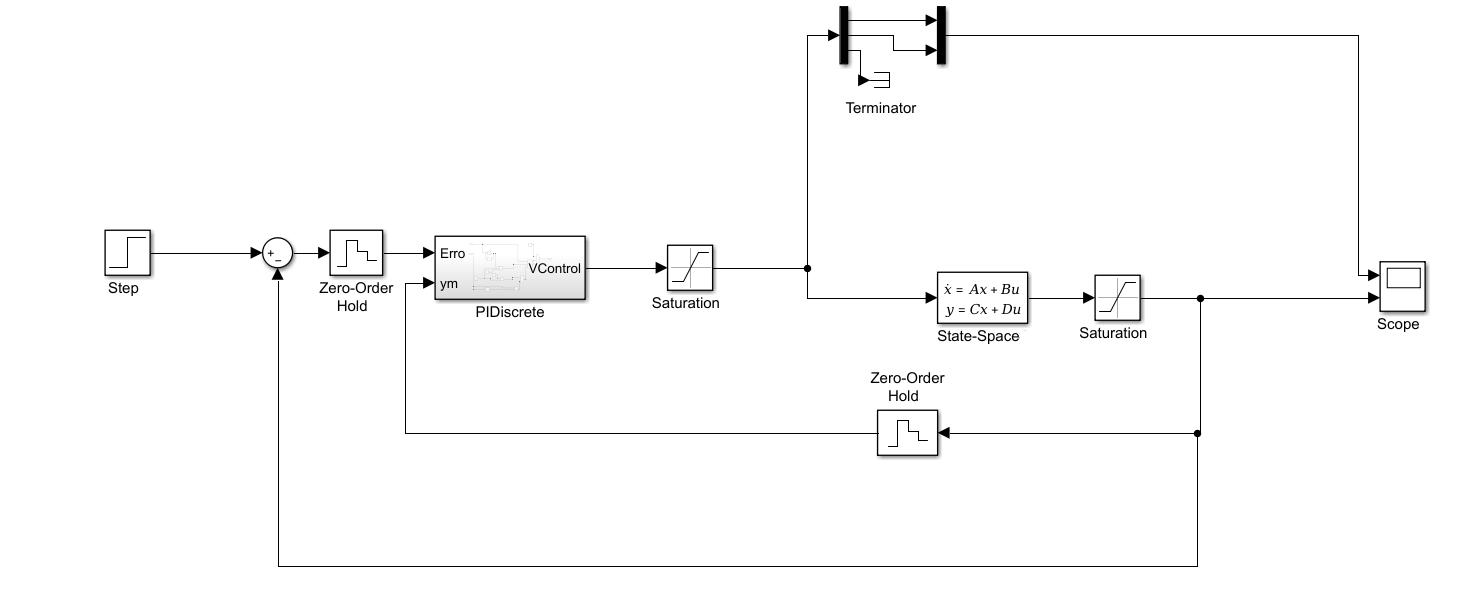
\includegraphics[page=1,width=1\textwidth]{img/diagrama.png} 
		\caption{Diagrama de Blocos}
\end{figure}
\begin{figure}[!htbp]
	\centering
      		 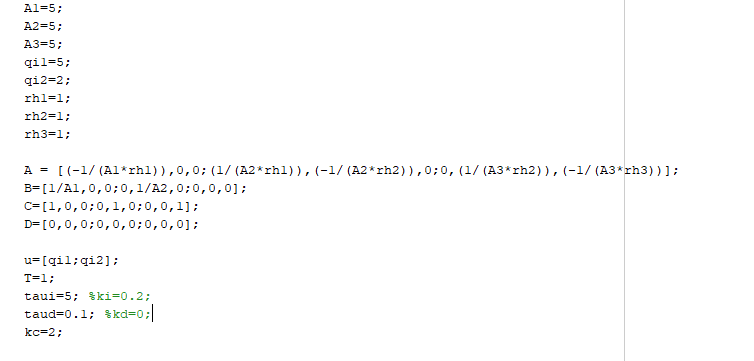
\includegraphics[page=1,width=0.8\textwidth]{img/parametros.png} 
		\caption{Inicialização}
\end{figure}

Após a criação do diagrama de blocos e da definição dos valores iniciais para as matrizes e constantes, seguiu-se para o estabelecimento das referências e o design do PID usando o algoritmo da velocidade (figura~\ref{fig:quatro}):
\begin{figure}[!htbp]
	\centering
      		 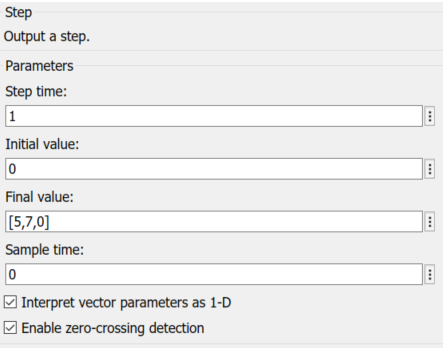
\includegraphics[page=1,width=1\textwidth]{img/step.png} 
		\caption{Estabelecimento das Referencias}
 	\label{fig:tres}
\end{figure}

\begin{figure}[!htbp]
	\centering
      		 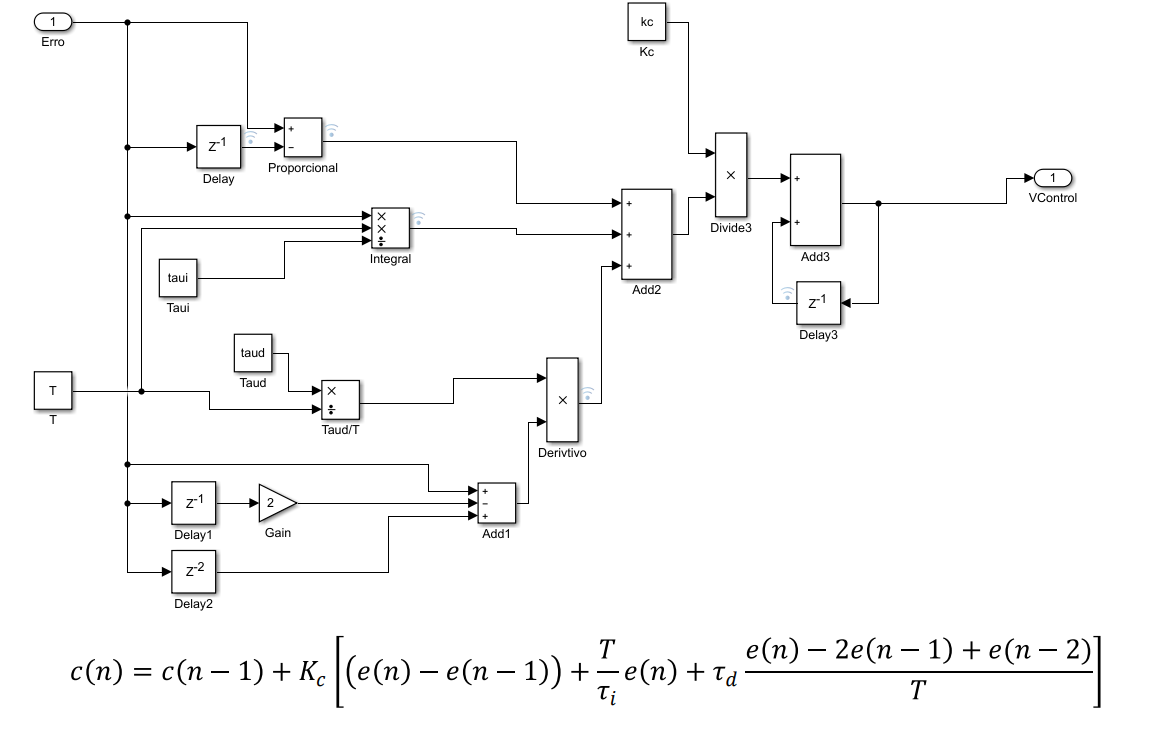
\includegraphics[page=1,width=0.8\textwidth]{img/pid2.png} 
		\caption{PIDVelocidade}
	\label{fig:quatro}
\end{figure}
\section{Simulação do PID}
Procedeu-se com a mesma metodologia do PID contínuo,  realizaram-se primeiro testes ao comportamento do controlador puramente proporcional. Inicialmente com Kp=1 (figura~\ref{fig:um}), tal como no PID contínuo, as entradas q1 e q2 começam com valores muito elevados, que apenas têm um limite devido a um bloco de saturação usado para simular as limitações físicas do sistema. Mas, em ambiente discreto isto apresenta um problema conhecido: verificou-se a presença de  \textbf{saltos derivativos}. \\ 
Seguidamente verifica-se que, tal como o PID contínuo, com apenas ganho proporcional o sistema é incapaz de alcançar as referências.\\ Após a alteração progressiva dos ganhos (kp, ki e kd) reparou-se que o sistema, como era de esperar, comporta-se da mesma forma que o contínuo e para evitar alguma redundância na informação, passar-se-á para os resultados mais notáveis.\\ Também se verificou que não havia diferença notável entre usar o algoritmo de posição, de velocidade e de posição modificado (figura ~\ref{}). O controlo ótimo foi encontrado no algoritmo de velocidade modificado.\\
A implementação de uma componente integral também permite a correção dos saltos derivativos pois permite o uso de uma versão modificada do algoritmo da velocidade (figura~\ref{fig:dois}). Isto é um detalhe importante \textbf{o algoritmo da velocidade modificado não funciona sem componente integral} pois se se analisar a equação na figura~\ref{fig:dois} verifica-se que a componente integral é a única que é influenciada pelo erro, todas as outras utilizam a medição da variável anterior que, se o ki for 0, será sempre 0 logo sem componente integral o algoritmo modificado não tem resposta.
\begin{figure}[!htbp]
	\centering
      		 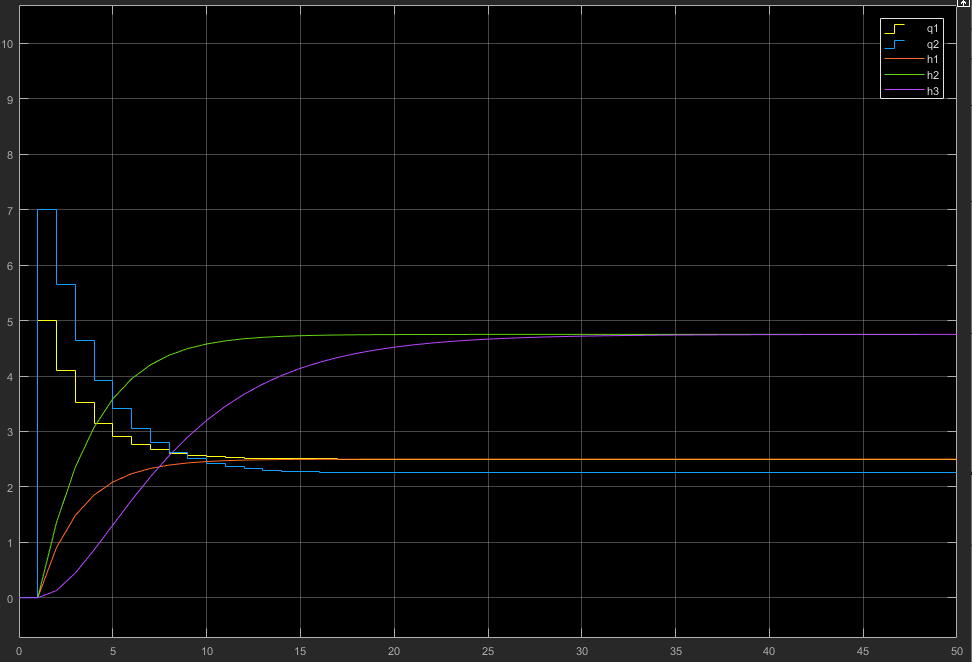
\includegraphics[page=1,width=1\textwidth]{img/puramenteP.png} 
		\caption{Kp=1}	
		\label{fig:um}
\end{figure}

\begin{figure}[!htbp]
	\centering
      		 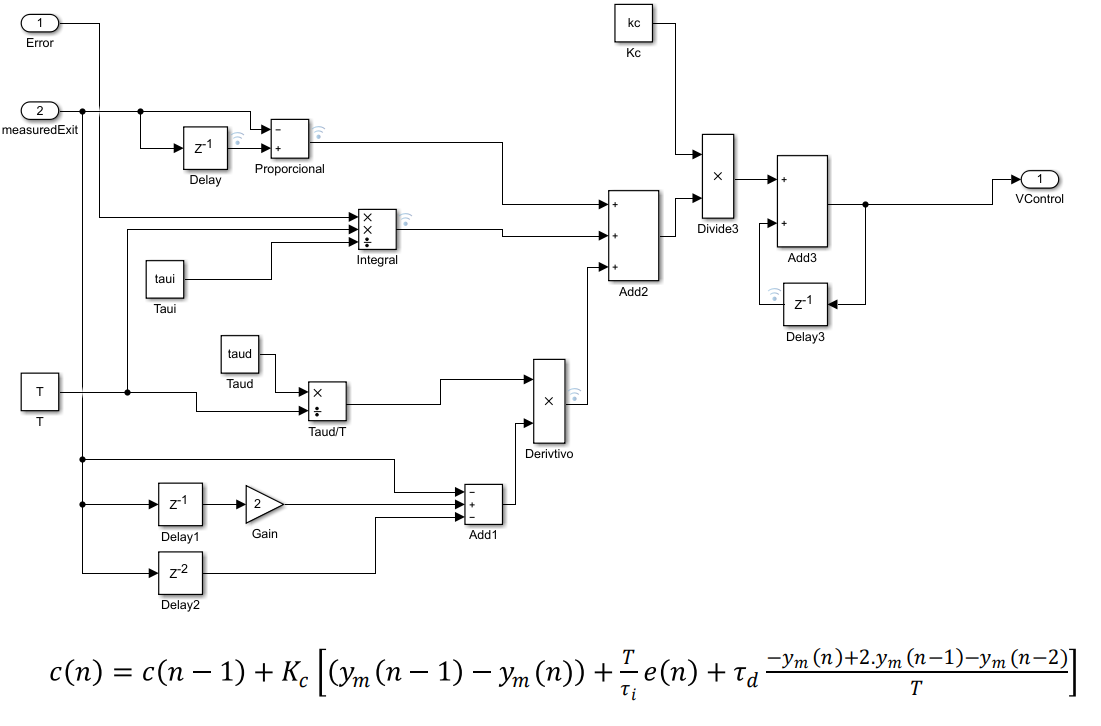
\includegraphics[page=1,width=1\textwidth]{img/pid.png} 
		\caption{Algoritmo de Velocidade Modificado}	
		\label{fig:dois}
\end{figure}

\newpage

Estabelecendo agora Ki=0.2,Kp=2, kd=0.1 e um sample time de 1s:

\begin{figure}[!htbp]
	\centering
      		 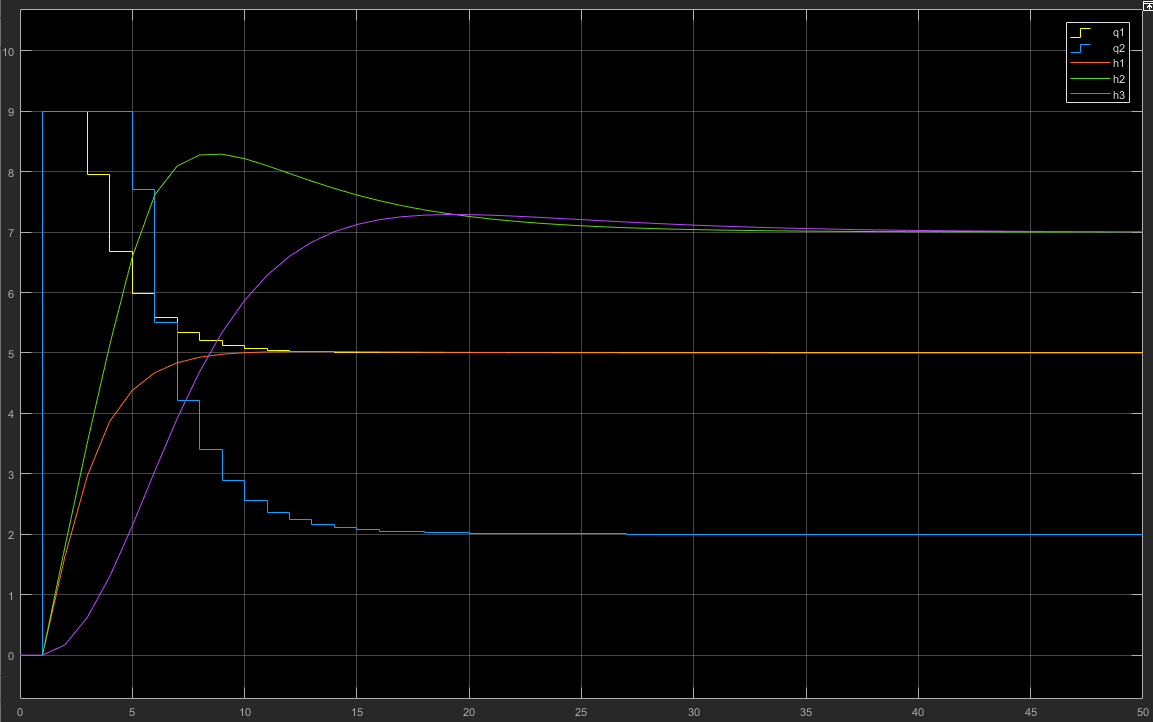
\includegraphics[page=1,width=1\textwidth]{img/new.png} 
		\caption{Resposta dos Algoritmos de Velocidade, Posição e Posição Modificado}	
		\label{pos}
\end{figure}

\begin{figure}[!htbp]
	\centering
      		 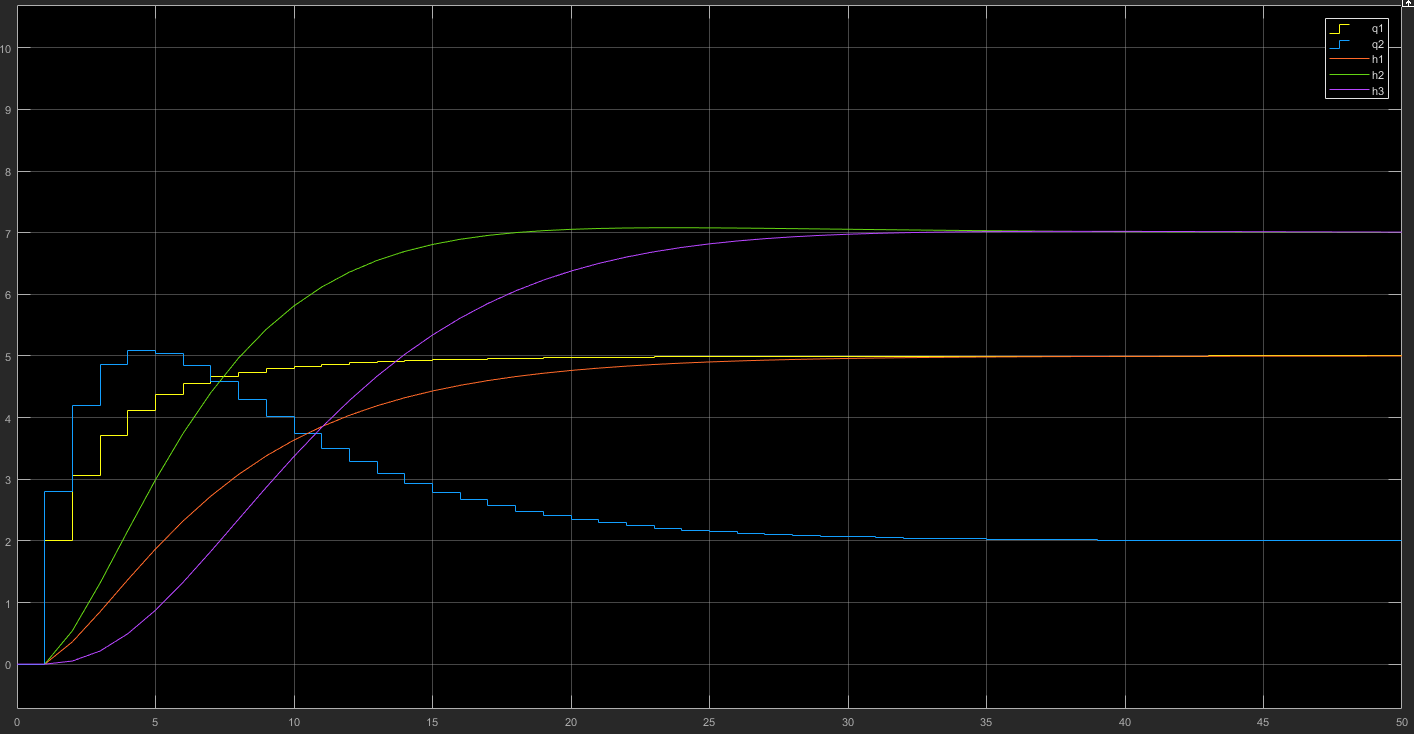
\includegraphics[page=1,width=1\textwidth]{img/full.png} 
		\caption{Resposta do Algoritmo de Velocidade Modificado}	
	\label{vel}
\end{figure}
Na figura~\ref{pos} com as novas componentes implementadas repara-se que os saltos derivativos mantiveram-se e nota-se ainda um overshoot sunbstancial que poderá ser consequência desses saltos juntamente com o efeito a componente integral, de qualquer das formas os saltos derivativos apresentam um problema para o sistema e devem ser corrigidos usando o algoritmo da velocidade modificado.

O caso ótimo do PID contínuo (figura ~\ref{vel}) é melhorado pelo algoritmo do PID discreto. Os saltos derivativos foram eliminados: as saídas do controlador vão aumentando progressivamente em vez de começarem imediatamente no valor máximo (ação que pode causar estragos ao sistema) ainda que ao custo da diminuição da velocidade do sistema. É de salientar que apesar da velocidade ter diminuído o sistema foi capaz de controlar as variáveis sem overshoot ou oscilações notáveis.

\section{Alteração do Sample Time}
A escolha do período de amostragem é um dos passos essencias para um bom controlo em ambiente discreto. Para este sistema nota-se que até 1s de T (figura~\ref{vel})o controlo não apresenta riscos para o sistema sendo que as entradas q1 e q2 não são forçadas a alcançar valores altos subitamente e as alturas dos tanques atingem a referência. A partir de T=2 (figura~\ref{t2}) nota-se que as entradas já têm saltos possivelmente perigosos mas ainda não apresenta problemas em termos de alcançar a referência.\\
Para T=3 (figura~\ref{t3}) os saltos das entradas pioram e nota-se alguma dificuldade no controlo das alturas, embora ainda alcançem as referências e se mantenham lá embora com alguma oscilação.
Para T=4 (figura~\ref{t4}) já se nota grandes dificuldades no controlo, o sistema é incapaz de se manter nas referências e as entradas apresentam saltos de grande magnitude, sendo por isso um perigo para o sistema.

\begin{figure}[!htbp]
	\centering
      		 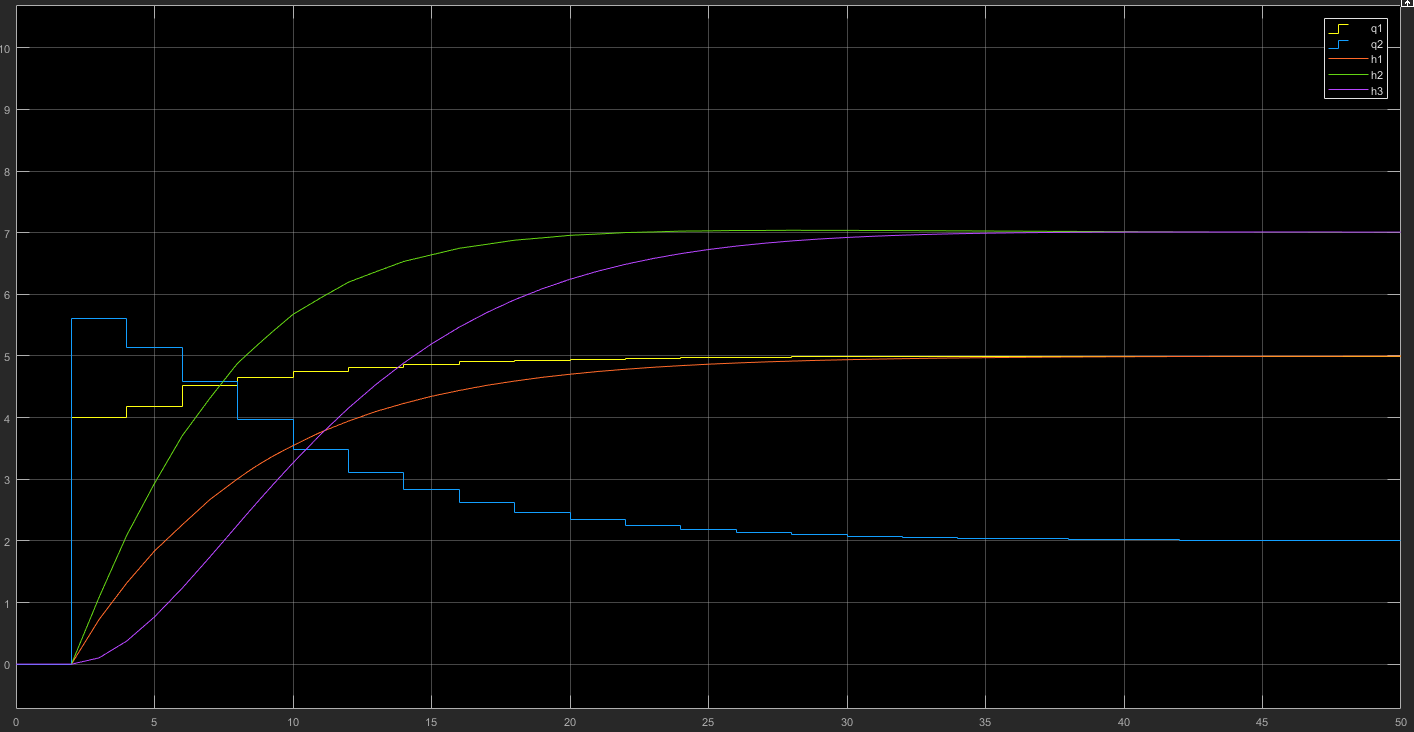
\includegraphics[page=1,width=1\textwidth]{img/t2.png} 
		\caption{Resposta do Algoritmo de Velocidade Modificado com T=2}	
	\label{t2}
\end{figure}

\begin{figure}[!htbp]
	\centering
      		 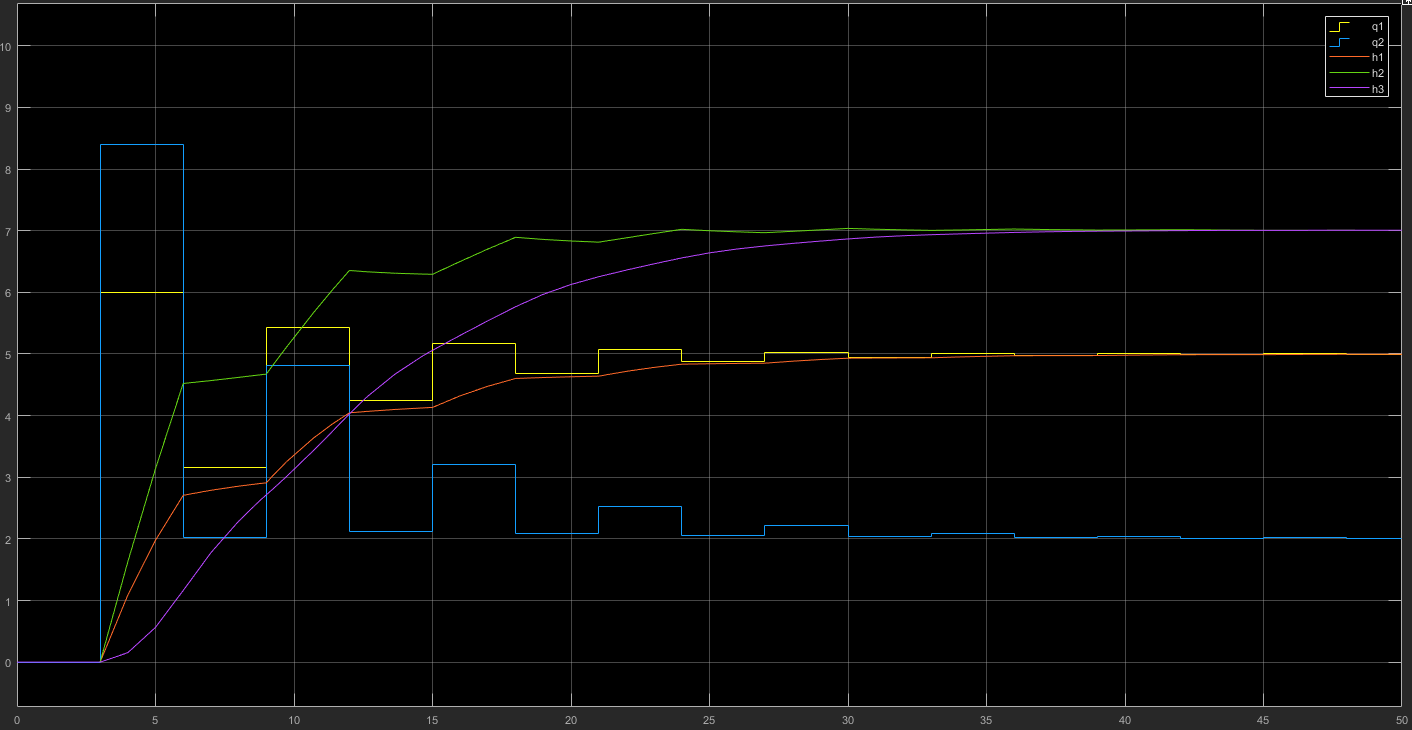
\includegraphics[page=1,width=1\textwidth]{img/t3.png} 
		\caption{Resposta do Algoritmo de Velocidade Modificado com T=3}	
	\label{t3}
\end{figure}


\begin{figure}[!htbp]
	\centering
      		 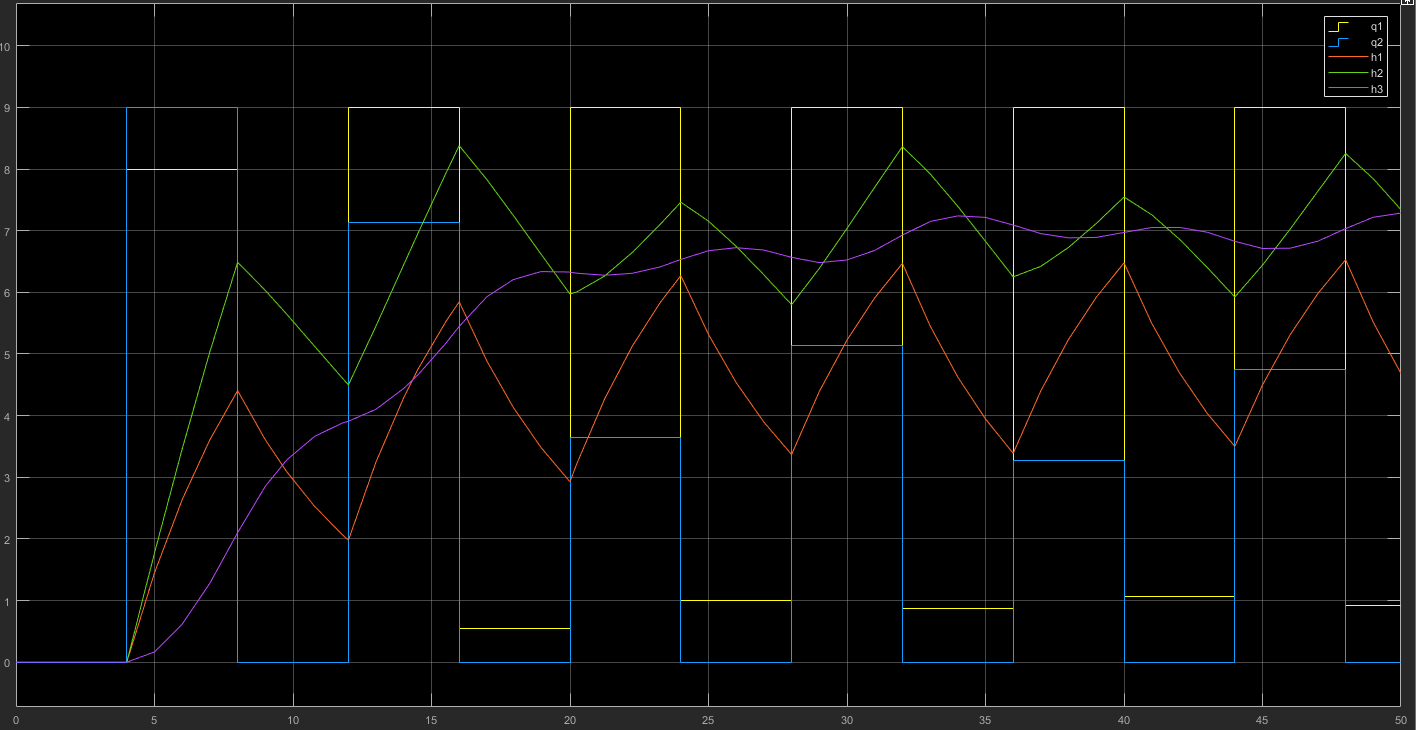
\includegraphics[page=1,width=1\textwidth]{img/t4.png} 
		\caption{Resposta do Algoritmo de Velocidade Modificado com T=4}	
	\label{t4}
\end{figure}
\newpage
\section{Conclusões}
\begin{itemize}
\item A simulação ideal do PID contínuo foi melhorada pelo PID discreto, a correção dos saltos das entradas no sistema diminuem a possibilidade de estragos neste.
\item Neste sistema os algoritmos de posição, velocidade e posição modificado apresentam respostas sem grandes diferenças umas em relação às outras.
\item Neste sistema o algoritmo ideal é o de velocidade modificado pois resolve o problema das entradas q1 e q2 terem uma variação de caudal muito grande em muito pouco tempo e assim diminui riscos de segurança.
\item O período de amostragem não pode ser 4 ou superior pois com esse T não há controlo e o sistema comporta-se melhor com T menor ou igual a 1.
\end{itemize}
\end{document}